\section*{Physique (13 points)}
\section*{Exercice 1 (2,5 points) : Désintégration de Strontium 90}
Le Strontium ${ }_{38}^{90} \mathrm{Sr}$ est l'un des principaux noyaux se trouvant dans les déchets des réacteurs nucléaires électrogènes. ${ }_{38}^{90} \mathrm{Sr}$ se désintègre en Yttrium ${ }_{Z}^{A} \boldsymbol{Y}$ en émettant une particule $\boldsymbol{\beta}^{-}$. Il est très nocif quand la particule est inhalée ou ingérée. Le noyau ${ }_{38}^{88} S r$ est l'un des isotopes de l'élément Strontium.

\section*{Données:}
\begin{center}
\begin{tabular}{|l|l|l|l|l|l|}
\hline
Particule & ${ }_{38}^{90} \mathrm{Sr}$ & ${ }_{Z}^{A} Y$ & Électron & Proton & Neutron \\
\hline
Masse en ( $u$ ) & ,90773 & 89,90714 & 0,0005 & 1,00728 & 1,00866 \\
\hline
\multicolumn{4}{|l|}{Demi-vie de ${ }_{38}^{90} \mathrm{Sr}: \quad t_{1 / 2}=28,9$ ans} & \multicolumn{2}{|c|}{$1 u=931,5 \mathrm{MeV} . c^{-2}$} \\
\hline
\multicolumn{2}{|l|}{Energie de liaison du noyau ${ }_{38}^{88} \mathrm{Sr}$ :} & \multicolumn{2}{|r|}{$E_{\ell}\left({ }_{38}^{88} S r\right)=768,47 \mathrm{MeV}$} & \multicolumn{2}{|c|}{1 an $=365$ jours} \\
\hline
\end{tabular}
\end{center}

\begin{enumerate}
  \item Écrire l'équation de désintégration de ${ }_{38}^{90} S r$ en précisant les valeurs de $A$ et $Z$ du noyau fils ${ }_{Z}^{A} Y$.
  \item Calculer, en unité MeV , l'énergie de liaison $E_{\ell}\left({ }_{38}^{90} \mathrm{Sr}\right)$ du noyau ${ }_{38}^{90} \mathrm{Sr}$.
  \item Déterminer, en justifiant, le noyau le plus stable parmi ${ }_{38}^{90} S r$ et ${ }_{38}^{88} S r$.
  \item Un échantillon de Strontium 90 a une activité initiale $a_{0}=5,11.10^{12} \mathrm{~Bq}$ à l'instant $t_{0}=0$.\\
4.1. Calculer le nombre $N_{0}$ des noyaux présents initialement dans cet échantillon.\\
4.2. Déterminer l'instant $t_{1}$ pour lequel l'activité de cet échantillon devient $a_{1}=10 \% a_{0}$.
\end{enumerate}




\section*{Exercice 2 (5 points) : Dipôle RC - Circuit RLC série}
Le dipôle $\boldsymbol{R C}$ et le circuit $\boldsymbol{R} \boldsymbol{L} \boldsymbol{C}$ série sont largement utilisés pour modéliser et analyser divers phénomènes électriques et électroniques. Ainsi, le dipôle $\boldsymbol{R C}$ permet de mettre en évidence la charge et la décharge d'un condensateur, alors que le circuit $\boldsymbol{R} \boldsymbol{L} \boldsymbol{C}$ série est fondamental pour l'étude des oscillations électriques libres.\\
Cet exercice vise :

\begin{itemize}
  \item l'étude de la réponse d'un dipôle $R C$ à un échelon de tension ascendant ;
  \item l'étude des oscillations électriques libres dans un circuit $\boldsymbol{R} \boldsymbol{L} \boldsymbol{C}$ série.
\end{itemize}

On étudie la charge d'un condensateur de capacité $C$ par un générateur idéal de tension de force électromotrice $E$, à travers un conducteur ohmique de résistance $R$ et sa décharge à travers une bobine ( $L, r$ ).

\begin{figure}[h]
\begin{center}
  \includegraphics[alt={},max width=\textwidth]{f47096eb-5ae7-4c60-ab2f-f9822564c423-3_371_463_2323_1500}
\captionsetup{labelformat=empty}
\caption{Figure 1}
\end{center}
\end{figure}

\section*{1. Réponse d'un dipôle $\boldsymbol{R} \boldsymbol{C}$ à un échelon de tension ascendant}
À l'instant $t=0$, on place l'interrupteur $K$ en position 1 (Figure 1).\\
La figure 2 indique l'évolution temporelle de la tension $u_{C}$ aux bornes du condensateur, et celle de la tension $u_{R}$ aux bornes du conducteur ohmique.\\
Donnée : $R=32 k \Omega$\\
1.1. Parmi les courbes (1) et (2), quelle est celle qui représente $u_{C}(t)$ ? Justifier.\\
1.2. Déterminer graphiquement la valeur de la force électromotrice $E$.\\
1.3. La constante de temps $\tau$ est la durée au bout de laquelle la charge du condensateur atteint $63 \%$ de sa charge maximale.\\
Déterminer graphiquement la valeur de $\tau$.\\
1.4. Vérifier que $C=47 \mu F$.

\begin{figure}[h]
\begin{center}
  \includegraphics[alt={},max width=\textwidth]{f47096eb-5ae7-4c60-ab2f-f9822564c423-4_540_803_504_1192}
\captionsetup{labelformat=empty}
\caption{Figure 2}
\end{center}
\end{figure}

1.5. L'expression de la tension $u_{C}$ est $u_{C}(t)=E$. $\left(1-e^{-t / \tau}\right)$.

Recopier, sur votre copie, le numéro de la question et choisir la lettre correspondante à la proposition vraie.\\
L'expression numérique de la charge $q(t)$ (en coulomb) du condensateur est :

\begin{center}
\begin{tabular}{|c|c|c|c|}
\hline
$\mathbf{A}$ & $q(t)=6.10^{-4} \cdot\left(1-e^{-1,5 . t}\right)$ & $\mathbf{B}$ & $q(t)=2,82.10^{-4} \cdot\left(1-e^{-0,67 . t}\right)$ \\
\hline
$\mathbf{C}$ & $q(t)=2,82.10^{-4} \cdot\left(1-e^{-666,7 . t}\right)$ & $\mathbf{D}$ & $q(t)=6 .\left(1-e^{-0,67 . t}\right)$ \\
\hline
\end{tabular}
\end{center}



\section*{2. Oscillations électriques libres dans un circuit $\boldsymbol{R} \boldsymbol{L} \boldsymbol{C}$ série}
Le condensateur ayant acquis sa charge maximale $q_{\max }$. Lorsqu'on bascule l'interrupteur en position 2 (Figure 1) à un instant $t_{0}=0$ choisi comme nouvelle origine de temps, le condensateur se décharge. La figure 3 représente l'évolution temporelle de la tension $u_{C}(t)$.\\
Donnée : $r=8,6 \Omega$\\
2.1. Établir l'équation différentielle vérifiée par la tension $u_{C}$.\\
2.2. Nommer le régime d'oscillation obtenu.\\
2.3. Déterminer graphiquement la valeur de la pseudo-période $T$ des oscillations.\\
2.4. On considère que la pseudo période $T$ est égale à la période propre $T_{0}$ de l'oscillateur $L C$.\\
Déduire la valeur de l'inductance $L$ de la bobine. (on prend ( $\pi^{2}=10$ )).

\begin{figure}[h]
\begin{center}
  \includegraphics[alt={},max width=\textwidth]{f47096eb-5ae7-4c60-ab2f-f9822564c423-4_487_864_1722_1117}
\captionsetup{labelformat=empty}
\caption{Figure 3}
\end{center}
\end{figure}

2.5. Calculer la variation de l'énergie totale $\Delta \mathscr{E}$ du circuit, entre les deux instants $t_{0}=0$ et $t_{1}=2 T$. Expliquer de point de vue énergétique le résultat obtenu.\\
2.6. Pour entretenir les oscillations électriques dans le circuit, on monte en série avec le condensateur et la bobine précédemment utilisés, un générateur ( $G$ ) qui délivre une tension $u_{G}(t)$ proportionnelle à l'intensité du courant électrique $u_{G}(t)=k . i(t)$ avec $k$ une constante (Figure 4).\\
2.6.1. Établir l'équation différentielle vérifiée par la charge $q(t)$ du condensateur.

\begin{figure}[h]
\begin{center}
  \includegraphics[alt={},max width=\textwidth]{f47096eb-5ae7-4c60-ab2f-f9822564c423-4_318_314_2316_1644}
\captionsetup{labelformat=empty}
\caption{Figure 4}
\end{center}
\end{figure}

2.6.2. Déterminer la valeur de $k$ pour que le circuit soit siège des oscillations électriques périodiques.



\section*{Exercice 3 (5,5 points): Mouvement d'un solide - Système oscillant (solide - ressort)}
Le mouvement des systèmes mécaniques est régi par les lois de la mécanique. Pour certains systèmes déformables ou le solide est soumis à une force de rappel comme celle exercée par le ressort, le système peut avoir un mouvement oscillatoire amorti ou non amorti qui peut être analysé suite à une étude dynamique ou énergétique.\\
Cet exercice vise :

\begin{itemize}
  \item l'étude du mouvement d'un solide lancé sur un plan horizontal ;
  \item l'étude du mouvement oscillatoire d'un système (solide - ressort).
\end{itemize}

\section*{Les parties 1 et 2 sont indépendantes}
\section*{Partie 1: Mouvement d'un solide sur un plan horizontal}
\begin{minipage}{0.65\linewidth}
    Dans un jeu de lancement sur un rail $AB$ rectiligne horizontal, un solide
    $\mathrm{(S_{0})}$ de masse $m_{0}$ et de centre d'inertie $G$ est lancé à
    partir d'une position $A$ avec une vitesse initiale $\vec{v}_{0}$
    horizontale pour atteindre une cible $\mathrm{(C)}$ qui se trouve en $B$ à
    la distance $d=AB$
    (Fig.~\ref{fig:2bac_svt_national_2025_normale_phys_ex3_1}).
    
    Le mouvement de $\mathrm{(S_{0})}$ sur le rail $AB$ se fait avec des
    frottements modélisés par une force $\vec{f}$ constante de sens opposé au
    sens du vecteur vitesse.
\end{minipage}
\hfill
\begin{minipage}{0.34\linewidth}
    \begin{figure}[H]
        \centering
        \begin{tikzpicture}[]
            \Sol{5cm}{3mm}{sol}
            \node[solide={7mm/7mm},anchor=south west] (S) at (sol.north west) {};
            \node[point,label={[above=3mm]:$A$}] (A) at (S.center) {};
            \draw[->] (A.center) -- ++(2,0)
                node[anchor=south east,inner xsep=0pt] {$\vec{v}_{0}$};
            \draw[->,thick] (A.center) -- ++(1,0)
                node[anchor=south east,inner xsep=0pt] {$\ex$};
            \node[minimum width=1mm,minimum height=1cm,anchor=south east,
                inner xsep=0pt,fill,label=right:$B$] (C) at (sol.north east) {};
            \node[anchor=south east,inner xsep=0pt,
                inner ysep=1pt] at (C.north east) {Cible $\mathrm{(C)}$};
        \end{tikzpicture}
        \caption{}
        \label{fig:2bac_svt_national_2025_normale_phys_ex3_1}
    \end{figure}
\end{minipage}
    
Pour étudier le mouvement de $G$ sur $AB$, on choisit le repère $(A,\ex)$ lié à
la Terre supposé galiléen.
    
À $t_{0}=0$~: $x_{G}=x_{A}=0$.

% \begin{donnees}
%     \begin{itemize}
%         \item $g=\qty{10}{\m\per\square\s}$~; $d=AB=\qty{1}{\m}$~;
%               $m_{0}=\qty{0.1}{\kg}$.
%     \end{itemize}
% \end{donnees}

\textbf{\textsc{Données~:}}
$g=\qty{10}{\m\per\square\s}$~; $d=AB=\qty{1}{\m}$~; $m_{0}=\qty{0.1}{\kg}$.

\begin{enumerate}
    \item En appliquant la deuxième loi de \textsc{Newton}, montrer que
          l'équation différentielle vérifiée par l'abscisse $x_{G}$ s'écrit~:
          $\frac{\mathrm{d}^{2}x_{G}}{\mathrm{d}t^{2}}=-\frac{f}{m_{0}}$.
    \item En déduire la nature du mouvement de $G$.
    \item L'équation de la vitesse $v_{G}(t)$ de $G$ s'écrit~:
          $v_{G}(t)=-1,5\cdot t+1,5$ ($\unit{\v}$).
          \begin{enumerate}
              \item Écrire l'expression numérique de l'équation horaire du
                    mouvement de $G$.
              \item Déterminer l'instant $t_{1}$ ou $\mathrm{(S_{0})}$ s'arrête.
              \item Déterminer la valeur de $f$.
              \item Le solide $\mathrm{(S_{0})}$ atteint-il la cible
                    $\mathrm{(C)}$~? Justifier.
          \end{enumerate}
    \item Déterminer, la valeur minimale $v_{0,\min}$ de la vitesse
          initiale avec laquelle $\mathrm{(S_{0})}$ doit être lancé pour qu'il
          atteigne la cible $\mathrm{(C)}$.
\end{enumerate}



\section*{Partie 2: Système oscillant (solide - ressort)}
\begin{minipage}{0.65\linewidth}
    On fixe un solide $\mathrm{(S)}$ de masse $m$ à un ressort $R$, à spires non
    jointives de masse négligeable et de raideur $K$, on obtient un oscillateur
    horizontal qui oscille sans frottements sur un rail horizontal.
    
    On étudie le mouvement du centre d'inertie $G$ du solide $\mathrm{(S)}$ dans
    un repère $(O,\ex)$ lié à la Terre supposé galiléen
    (Fig.~\ref{fig:solide_ressort}). À l'équilibre $x_{G}=x_{0}=0$.
\end{minipage}
\hfill
\begin{minipage}{0.34\linewidth}
    \begin{figure}[H]
        \centering
        \begin{tikzpicture}
    \node[inner sep=0pt,minimum width=4.5cm,minimum height=3mm,
        top color=black!70] (sol) {};
    % Axe xx'
    \coordinate (O) at ($(sol.south west)!.8!(sol.south east)$);
    \draw[-Latex] (sol.south west)
        node[below right,inner xsep=0pt] {$x^{\prime}$} -- (O)
        node[below=0.4mm] {$O$} -- (sol.south east) -- ++(0.7,0)
        node[below left,inner xsep=0pt,inner ysep=2mm] {$x$};
    % Fixed
    \node[inner sep=0pt,draw,minimum width=3mm,minimum height=7mm,
        anchor=south,pattern=north west lines,
        thick] (fix) at ([xshift=3mm,yshift=0.4pt]sol.north west) {};
    % Solide (S)
    \node[inner sep=0pt,draw,minimum width=7mm,minimum height=7mm,
        anchor=south,rounded corners=2pt,thick,label=$\mathrm{(S)}$,
        fill=lightgray] (S) at
        ([yshift=0.4pt]O |- sol.north) {};
        %([xshift=-6mm,yshift=0.4pt]sol.north east) {};
    \node[inner sep=1pt,circle,fill,
        label={[right=-0.8mm,font=\scriptsize]:$G$}] (G) at (S.center) {};
    \draw[{Rectangle[length=1pt,width=4pt]}-{Stealth[length=5pt]},
        thick] (O) -- ++(0.8,0)
        node[below left,inner xsep=0pt] {$\ex$};
    % Ressort
    \draw[decoration={
          coil,
          aspect=0.3,
          segment length=2.0mm,
          amplitude=2.4mm,
          pre length=1mm,
          post length=1mm},
          decorate,thick,black] (fix.east) -- (S.west);
\end{tikzpicture}

        \caption{}
        \label{fig:solide_ressort}
    \end{figure}
\end{minipage}

On écarte $\mathrm{(S)}$ de sa position d'équilibre d'une distance $X_{m}$ et on
l'abandonne sans vitesse initiale à l'instant $t_{0}=0$, le solide
$\mathrm{(S)}$ est alors animé d'un mouvement de translation rectiligne
sinusoïdal d'équation
${x_{G}(t)=X_{m}\cdot\cos\left(\frac{2\pi}{T_{0}}t+\varphi\right)}$.

\begin{minipage}[t][][t]{0.60\linewidth}
La courbe de la Fig.~\ref{fig:tdb_2bac_svt_national_2025_normale_phys_ex3_3}
donne le diagramme des espaces $x_{G}(t)$ obtenu.

\textbf{Données~:} $m=\qty{200}{\g}$
\begin{enumerate}
    \item Déterminer graphiquement la valeur de la période propre $T_{0}$ de
          l'oscillateur et celle de l'amplitude $X_{m}$ des oscillations.
    \item Écrire l'expression numérique de l'équation horaire du mouvement de
          $G$.
    \item On choisit l'état où le ressort n'est pas déformé comme état de
          référence de l'énergie potentielle élastique $E_{pe}$ et le plan
          horizontal contenant $G$ comme état de référence de l'énergie
          potentielle de pesanteur $E_{pp}$.

          La courbe de la
          Fig.~\ref{fig:tdb_2bac_svt_national_2025_normale_phys_ex3_4} donne le
          diagramme de l'énergie potentielle élastique $E_{pe}$ de l'oscillateur
          (solide - ressort).
          \begin{enumerate}
              \item Déterminer graphiquement la valeur maximale $E_{pe,\max}$ de
                    l'énergie potentielle élastique.
              \item Déduire la valeur de la raideur $K$ du ressort.
              \item Déterminer la valeur de l'énergie cinétique du solide
                    lorsque $G$ passe par la position d'élongation
                    ${x_{G}=\qty{0.02}{\m}}$.
          \end{enumerate}
\end{enumerate}
\end{minipage}
\hfill
\begin{minipage}[t][][t]{0.38\linewidth}
    \vspace{-5mm}
    \begin{figure}[H]
        \centering
        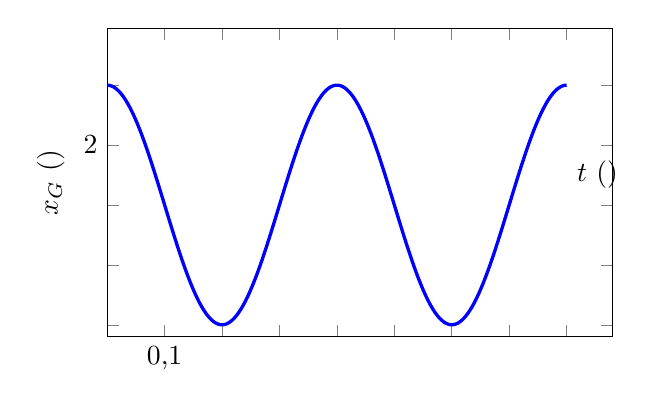
\begin{tikzpicture}
            \def\Xm{4}
            \def\T{0.4}
            \pgfmathpi\let\pi=\pgfmathresult
            \begin{axis}[
                    xmin=0,xmax=2.2*\T,
                    ymin=-4.4,ymax=5.9,
                    width=8cm,height=5.5cm,
                    trig format plots=rad,
                    xtick distance=0.1, ytick distance=2,
                    xticklabels={,,{0,1}}, yticklabels={,,,,{2}},
                    xlabel=$t~(\unit{\second})$, ylabel=$x_{G}~(\unit{\cm})$,
                    every axis x label/.append style={
                        at={(1.03,0.45)},anchor=south east,
                    },
                    minor tick num=0,
                ]
                \addplot[domain=0:2*\T,samples=200,very thick,blue]
                    {\Xm*cos(2*pi/\T*x)};
            \end{axis}
        \end{tikzpicture}
        \caption{}
        \label{fig:tdb_2bac_svt_national_2025_normale_phys_ex3_3}
    \end{figure}
    \begin{figure}[H]
        \centering
        \begin{tikzpicture}
            \def\K{50}
            \def\Xm{0.04}
            \begin{axis}[
                    xmin=-0.045,xmax=0.045,
                    ymin=0,ymax=55,
                    width=8cm,height=5.5cm,
                    xlabel=$x~(\unit{\meter})$,
                    ylabel=$E_{pe}~(\unit{\mJ})$,
                    every axis y label/.append style={
                        at={(0.55,0.95)},anchor=west,
                    },
                    scaled ticks=false,
                    xtick distance=0.01, ytick distance=10,
                    xticklabels={,,,,,,{0,01}}, yticklabels={,,{10}},
                    minor tick num=0,
                ]
                \addplot[domain=-\Xm:\Xm,samples=200,
                    very thick,blue] {0.5*\K*x^2*1e3}
                    coordinate[pos=0](A) coordinate[pos=1](B);
            \end{axis}
            \foreach \n/\a in {A/200,B/-20}{%
            \draw[very thick] ([yshift=-5mm]\n) -- ([yshift=5mm]\n);
            \foreach \f in {0.02,0.14,...,1}
                \draw[thick]
                    ($([yshift=-5mm]\n)!\f!([yshift=5mm]\n)$) -- ++(\a:.2);
            }
        \end{tikzpicture}
        \caption{}
        \label{fig:tdb_2bac_svt_national_2025_normale_phys_ex3_4}
    \end{figure}
\end{minipage}





